\begin{figure}[H]
\centering
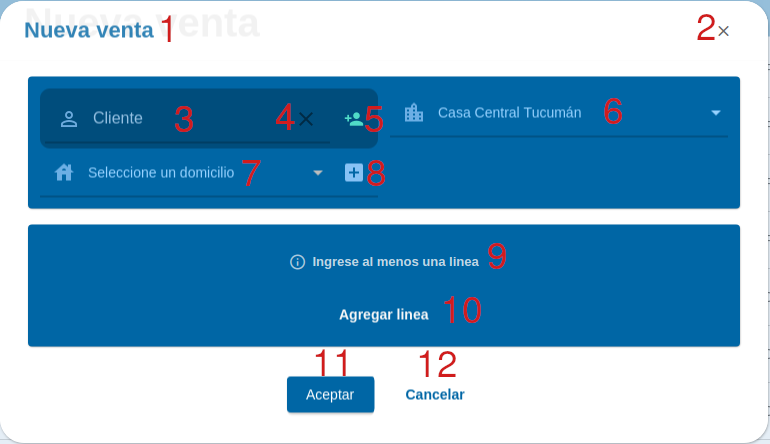
\includegraphics[width=\textwidth,height=\textheight,keepaspectratio]{Escenarios/AD-11-00}
\caption{Escenario - AD-11-00}
\label{fig:AD-11-00}
\end{figure}
Este es el escenario que permite a los usuarios crear y modificar ventas, el campo \textbf{AD-11-01} indicará la acción que se va a realizar, pudiendo ser 'Nueva venta' o 'Editar venta'. Con el botón \textbf{AD-11-02} se podrá cerrar la ventana y volver al escenario \textbf{AD-10-00}.
El campo \textbf{AD-10-03} permite al usuario indicar el cliente para el cúal se esta creando la venta o indicar el nuevo cliente en caso que se esté editando el presupuesto. Un click en botón \textbf{AD-10-04} eliminará la seleccion que se encuentre en el campo \textbf{AD-10-03}. El botón \textbf{AD-10-05} permite crear un nuevo cliente navegando al escenario \textbf{AD-29-00}. La lista desplegable \textbf{AD-10-06} permite al usuario indicar la ubicación en la cúal se esta creando la venta o bien modificar la misma. En la lista desplegable \textbf{AD-11-07} se mostrarán los domicilios del cliente seleccionado en el campo \textbf{AD-11-03}, de los cuales el usuario deberá elegir uno para la venta. El botón \textbf{AD-11-08} navega al escenario \textbf{AD-31-00} para crear un domicilio para el cliente.
El campo \textbf{AD-10-09} se muestra cuando la venta no tiene asociado ninguna linea de venta. El boton \textbf{AD-10-10} permite al usuario crear una linea de venta y asociarla a la venta, navega al escenario \textbf{AD-05-00}. Si el usuario hace click en el botón \textbf{AD-10-11} creará la venta y navegará al escenario \textbf{AD-13-00}, si hace click en el botón \textbf{AD-04-09} cerrará la ventana navegando al escenario \textbf{AD-10-00}.
\clearpage
